\documentclass{article}
\usepackage[dvipsnames]{xcolor}
\usepackage[paperwidth=20cm, paperheight=4.5cm, margin = 0cm, top=0.25cm]{geometry}

\usepackage{pgf}
\usepackage{tikz}
\usetikzlibrary{arrows,automata}
\usetikzlibrary{positioning}
\tikzstyle{source}  = 
[
	draw,circle,fill=black,thick,inner sep=0mm,minimum size=2mm
]

\tikzstyle{box}  =
[
	draw,rectangle,thick,inner sep=2mm,
	minimum width=8mm, minimum height=8mm
]

\tikzstyle{redbox} = 
[
	draw,rectangle,thick,inner sep=2mm,
	minimum width=8mm, minimum height=8mm,
	fill=red, opacity=0.3, text opacity=1, draw opacity=1
]

\tikzstyle{bluebox} = 
[
	draw,rectangle,thick,inner sep=2mm,
	minimum width=8mm, minimum height=8mm,
	fill=blue, opacity=0.3, text opacity=1, draw opacity=1
]

\tikzstyle{lgreenbox} = 
[
	draw,rectangle,thick,inner sep=2mm,
	minimum width=8mm, minimum height=8mm,
	fill=SpringGreen
]

\tikzstyle{bluestate}  = 
[
	state, draw=blue, line width=2pt,
	fill=LimeGreen
]

\tikzstyle{redstate}  = 
[
	state, draw=red, line width=2pt,
	fill=LimeGreen
]

\tikzstyle{violetstate}  = 
[
	state, draw=Violet, line width=2pt,
	fill=LimeGreen
]
 

\begin{document}
\begin{center}
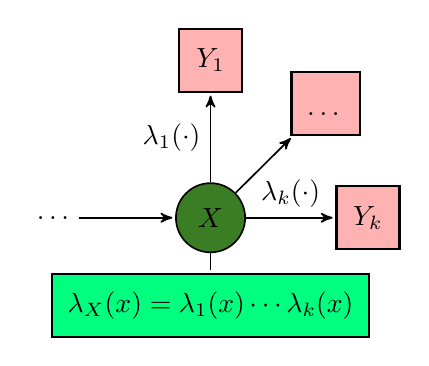
\begin{tikzpicture}[->,>=stealth',shorten >=1pt,auto,node distance=2.0cm,semithick]
                    
\node (X1) {$\ldots$}; 
\node[state, fill=OliveGreen](X2) [right of=X1] {$X$};
\node[redbox] (X3) [above of=X2] {$Y_1$};                   
\node[redbox](X4) [right=0.6cm of X3, yshift=-0.55cm] {$\ldots\rule{0pt}{2ex}$}; 
\node[redbox](X5) [right of=X2] {$Y_k$}; 

\node[lgreenbox][below=0.25cm of X2](P2){$\lambda_X(x)=\lambda_1(x)\cdots\lambda_k(x)$};               

\path
	(X1) edge (X2)
	(X2) edge node[left]{$\lambda_1(\cdot)$}(X3)
	(X2) edge (X4)
	(X2) edge  node[above]{$\lambda_k(\cdot)$} (X5);

\path
	(X2) edge[-] (P2);



\end{tikzpicture}
\end{center}

\end{document}
